\documentclass[acmtog]{acmart}
\usepackage{graphicx}
\usepackage{subfigure}
\usepackage{natbib}
\usepackage{listings}
\usepackage{bm}

\def\x{\mathrm{\mathbf{x}}}
\def\y{\mathrm{\mathbf{y}}}
\def\z{\mathrm{\mathbf{z}}}
\def\w{\omega}
\def\p{\mathrm{p}}
\def\pp#1#2{\p_{#1}\rightarrow\p_{#2}}

\definecolor{blve}{rgb}{0.3372549 , 0.61176471, 0.83921569}
\definecolor{gr33n}{rgb}{0.29019608, 0.7372549, 0.64705882}
\makeatletter
\lst@InstallKeywords k{class}{classstyle}\slshape{classstyle}{}ld
\makeatother
\lstset{language=C++,
	basicstyle=\ttfamily,
	keywordstyle=\color{blve}\ttfamily,
	stringstyle=\color{red}\ttfamily,
	commentstyle=\color{magenta}\ttfamily,
	morecomment=[l][\color{magenta}]{\#},
	classstyle = \bfseries\color{gr33n}, 
	tabsize=2
}
\lstset{basicstyle=\small\ttfamily}

% Title portion
\title{Final Project:\\ {Smoke Rendering}}

\author{ YiHeng Wu }

% Document starts
\begin{document}
\maketitle

\vspace*{2 ex}

\section{Section 1}

\section{Section 2}

\section{Implementation}
    The implementation is based on HW3 and HW4 of YiHengWu.
    It follows the PBRT naming style for variables and functions so that those who are familiar with PBRT will find it comfortable to read the code.\par
        The PBRT-style framework splits the tracer into independent parts: 
    shape, primitive, aggregate, sampler, distribution, scattering, material, texture, light, medium.
    These information accompanied with the camera are recorded in the scene settings.
    The scene is finally rendered by the integrator and an image is outputted.\par
        We assume that the readers are familiar with PBRT so we will only focus on medium, integrator and aggregate.

\subsection{Volume}
    See `medium/volume.h' and `medium/volume.cpp' for more details.\par
        The volume framework is based on OpenVDB, 
    thus a volume is simply a OpenVDB grid with some interfaces to access the internal value.
    A smoke can be mostly described by its density with a VDB float grid.
    A problem is that the grid is described in an unsigned integer coordinate (grid coordinate) so that
    rays should be transformed from the world coordinate to the grid coordinate before tracking.
    That is why `LocalToGrid()' is a necessary virtual function of `class Volume'.
\begin{lstlisting}
class Volume:
public:
    virtual Transform LocalToGrid() const = 0;
\end{lstlisting}
    We will focus on the child class `class VolumeFloatGrid' and its child class `class VolumeFloatKDTree'.\par
        The reason why we also need a KDTree is that 
    simply using the uniform grid for decomposition tracking will always result in bad performance 
    because the minimum value of grid, which is chosen as $\mu_t^c$, is always very small.
    So we use a KDTree to split the grid into blocks where the minimum value inside each block is expected to be higher.
    Our implementation of the KDTree is based on the article introduced above.
\begin{lstlisting}
class VolumeFloatGrid : public Volume;
class VolumeFloatKDTree : public VolumeFloatGrid;
\end{lstlisting}

\subsubsection{Grid}
        The implementation of `class VolumeFloatGrid' is quite simple.
    It simply provides interfaces between our framework and OpenVDB data structure.
    Information about the grid including the max and min value and the boundary are recorded as fields to enable fast accessing.

\subsubsection{KDTree}
        The KDTree is the child class of the grid, with node-level fields including the max and min value, split axis and split position.
    Information about a node is compressed and recorded into 64 bits.
    The format of the tree is shown here.
\begin{figure}[H]
    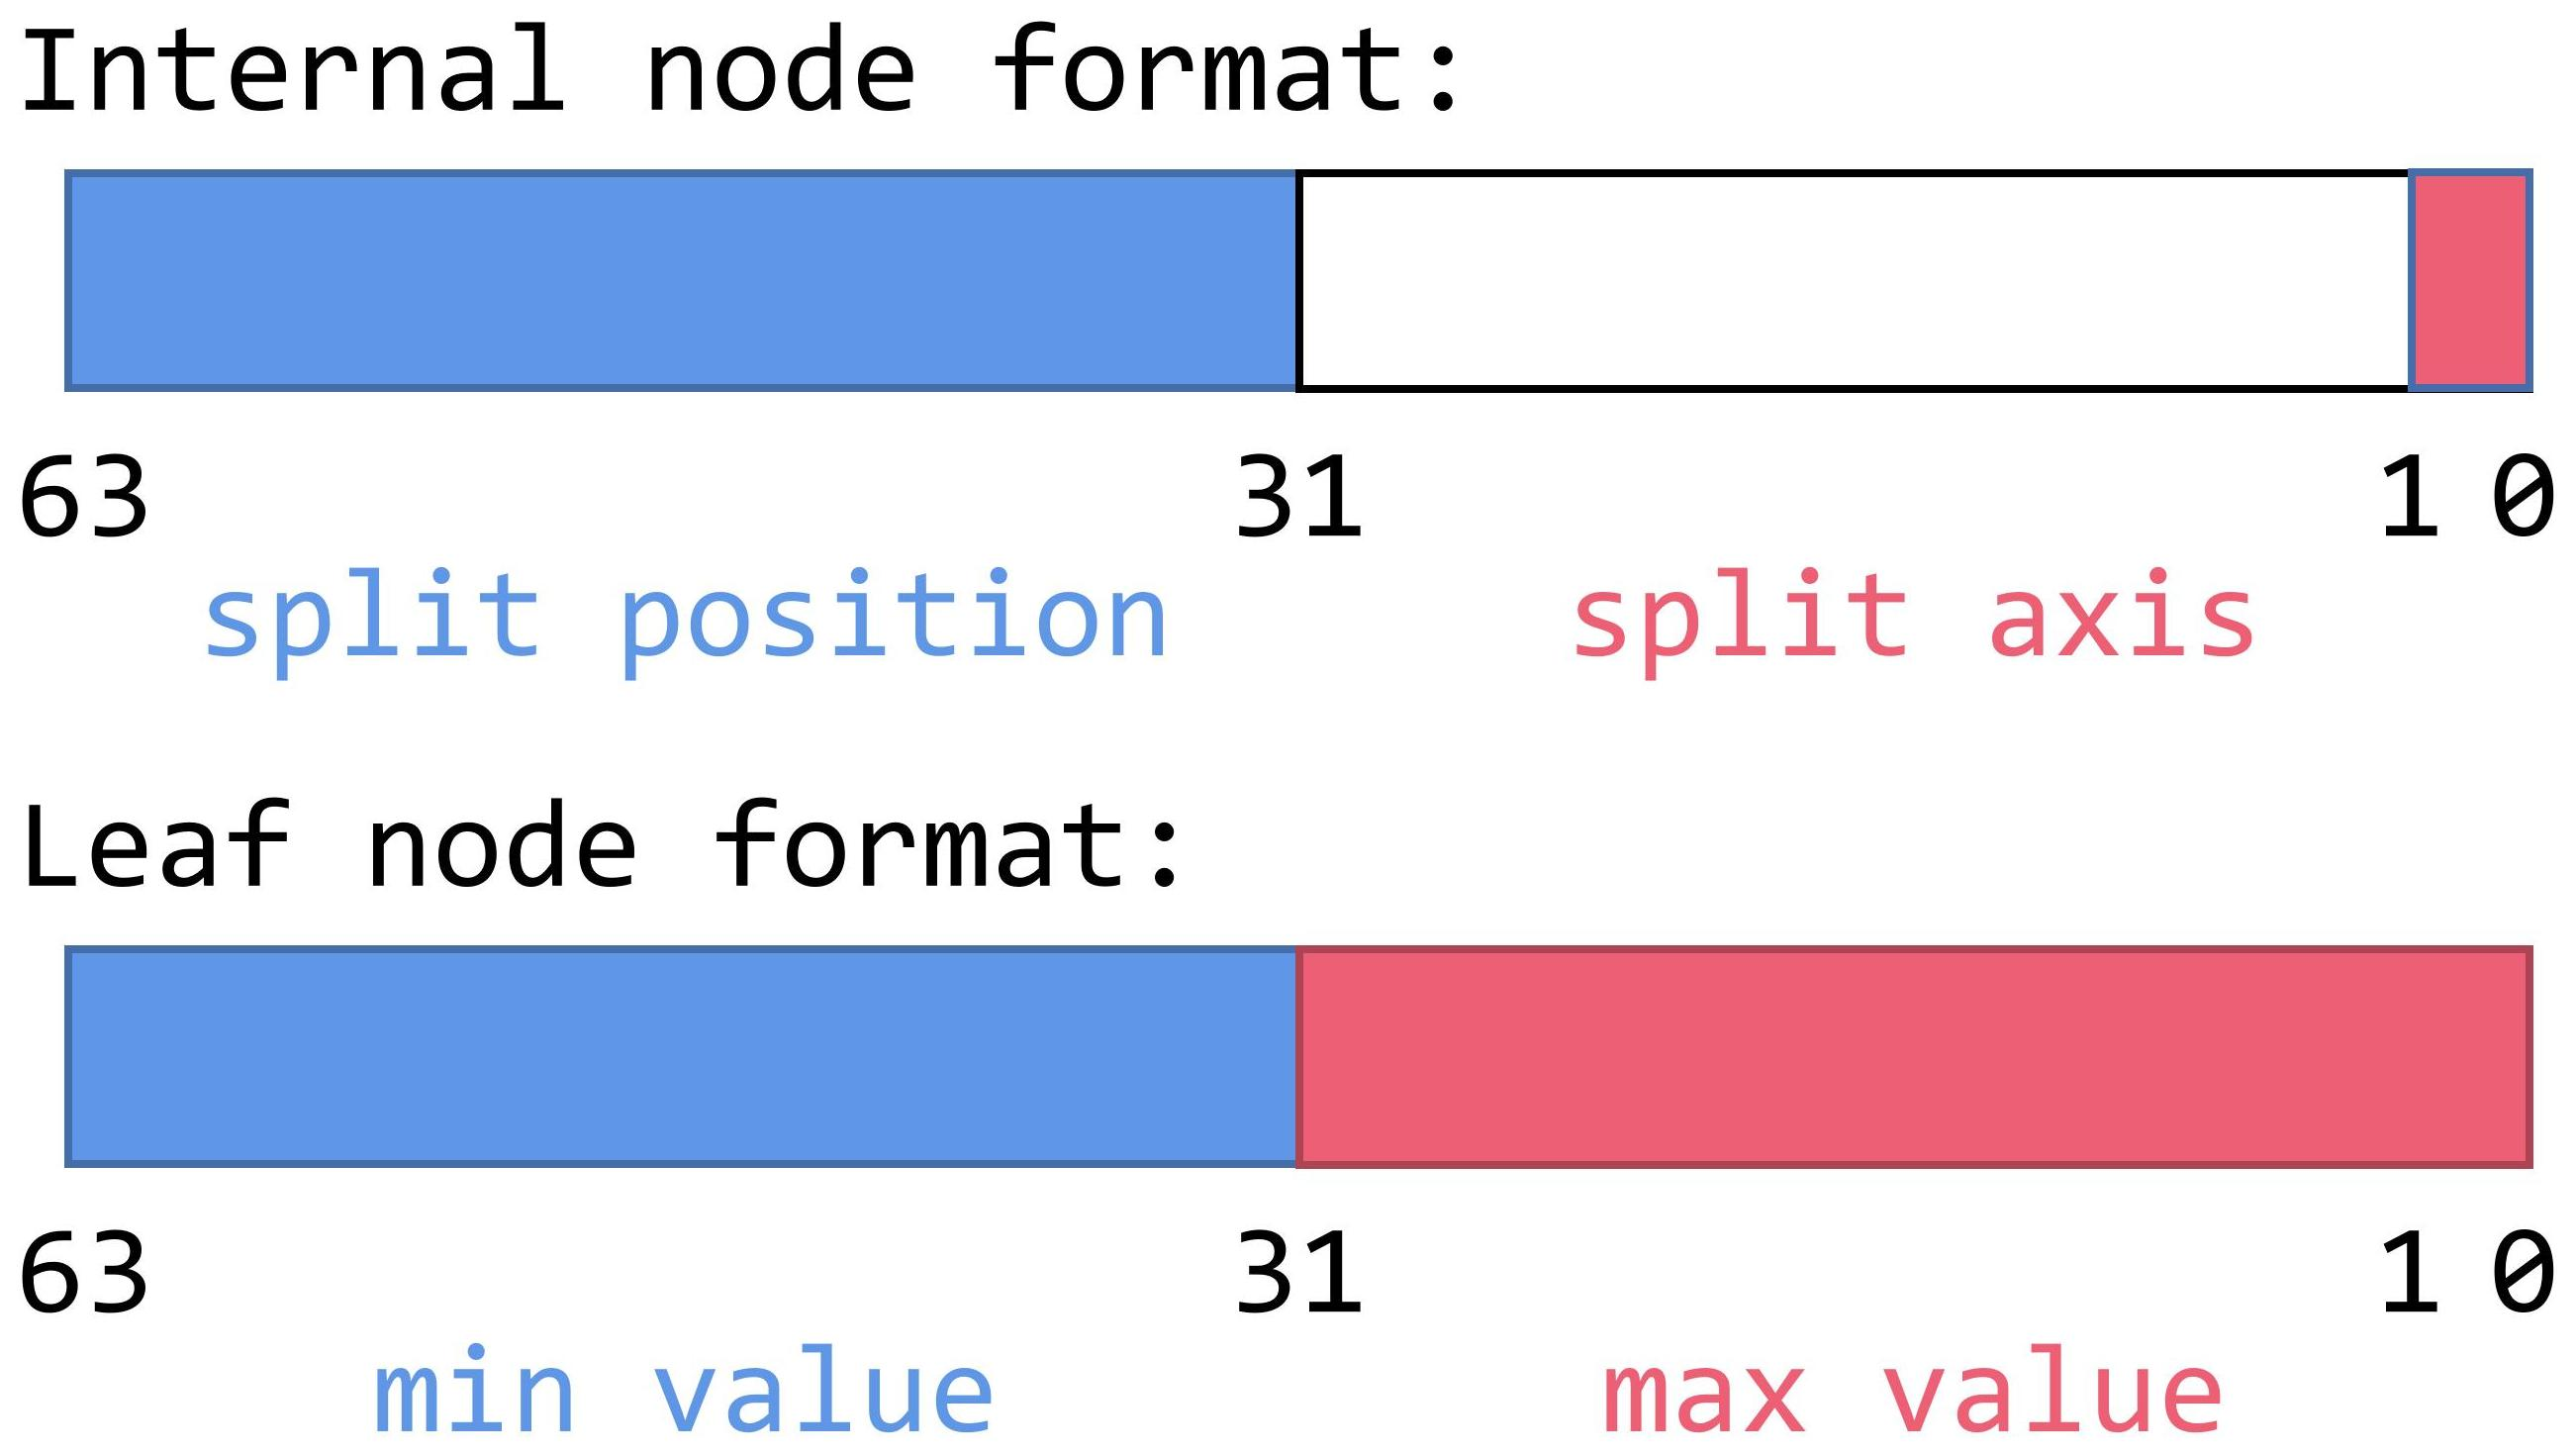
\includegraphics[scale=0.065]{pictures/kdTree format.png}
    \centering
    \caption{KDTree node format.}
\end{figure}
        The lowest two bits (split axis) is used to indicate whether a node is a internal or leaf node.
    For internal nodes, split axis $\in { 0, 1, 2 }$ indicating ${ x, y, z }$ axis.
    For leaf nodes, the lowest two bits are fixed to $3$.\par
        You may have noticed that split axis shares two bits with max value so that
    for leaf nodes, the lowest two bits of the max value is always `0b11', 
    which results in some acceptable errors but achieves great speedup.\par
        You may also have noticed that parent nodes do not record the index of their child nodes.
    This makes our kdTree different from PBRT.
    We compressed the kdTree into a heap where children of node at array index $i$ are located at $i<<1$ and $(i<<1)+1$.
    We chose this design to compress the node into 64-bits, making it more cache-friendly for 64-bit-cacheline systems.\par
        Following this format, `class VolumeFloatKDTree' provides 4 inline functions to
    get split axis, split position of internal nodes and max, min value of leaf nodes.
    Here shows the interfaces, where `idx' is the index of the kdTree array with 64-bit stride.
\begin{lstlisting}
class VolumeFloatKDTree : public VolumeFloatGrid:
public:
    inline int KDTreeSplitAxis(int idx) const;
    inline int KDTreeSplitPos(int idx) const;
    inline int KDTreeMaxValue(int idx) const;
    inline int KDTreeMinValue(int idx) const;
private:
    void* kdTree;
\end{lstlisting}
        Building of the KDTree is based on the article introduced above.
    Since the implementation is simple, it will not be discussed here.

\subsection{Medium}
    See `medium/medium.h', `medium/medium.cpp' for more details.\par
        This section will focus on the interface design of the medium system.
    Readers can skip this part if they are familiar with PBRT.\par
        As we have fully explained, the volume path tracing procedure primarily needs 3 building blocks:
    sampling scattering distance, evaluating transmittance and sampling scattering direction.\par
\subsubsection{Sample Distance}
        Weighed delta tracking and weighed decomposition tracking are used.
    Since these two solutions are based on reject sampling, a random number generator (or a sampler in our framework) is needed.
    The current weight is also given as a parameter, which will be updated during samples.
    Sampling results including the position is recorded in a `MediumInteraction'.
    Here is the interface.
\begin{lstlisting}
class Medium:
public:
    virtual Spectrum Sample(
        const Ray& rayWorld,  // World-coord ray
        Sampler& sampler,     // Random generator
        Spectrum* weigh,      // Weighed tracking
        MediumInteraction* mi // Sampling results
    ) const = 0;
\end{lstlisting}
    The return value is a spectrum used to update $\beta$ in integrators.
    It will be explained in detail later.
\subsubsection{Evaluate Transmittance}
        Our implementation of evaluating transmittance is based on radio tracking and residual radio tracking, thus a sampler is also needed.
    We follow the rule that the transmittance to evaluate is between $t = 0$ and $t = \mathrm{rayWorld.tMax}$.
    Here is the interface.
\begin{lstlisting}
class Medium:
public:
    virtual Spectrum Tr(
        const Ray& rayWorld, // World-coord ray
        Sampler& sampler,    // Random generator
    ) const = 0;
\end{lstlisting}
\subsubsection{Sample Direction}
        We simply sample the HenyeyGreenstein phase function so that the interface is similar to PBRT.
\begin{lstlisting}
class PhaseFunction:
public:
    virtual Float P(
        const Vector3f& wo, // Omega out
        const Vector3f& wi  // Omega in
    ) const = 0;
    virtual Float Sample_P(
        const Vector3f& wo, 
        Vector3f* wi, 
        const Point2f& samples
    ) const = 0;
class HenyeyGreenstein : public PhaseFunction;
\end{lstlisting}

\subsection{Surface}
    See `medium/medium.h', `medium/medium.cpp' for more details.\par
        To combine surface rendering and volume rendering, 
    it is necessary to know whether the ray is travelling through air or inside some medium such as smoke.
    The simplest approach is assigning every primitive a surface, 
    which records the medium outside the primitive surface and inside the primitive surface.
\begin{lstlisting}
class Surface:
public:
    const Medium* mediumIn; // Medium inside
    const Medium* mediumOu; // Medium outside
\end{lstlisting}
    Then every geometric primitive should be constructed with a surface instance.
\begin{lstlisting}
class GeometricPrimitive : public Primitive:
public:
    const Surface surface;
\end{lstlisting}
    When `GeometricPrimitive::Intersect()' is called, surface information should be recorded in a `SurfaceInteraction' instance.
    So `class SurfaceInteraction' should also contain a `Surface' instance as its field.
\begin{lstlisting}
class SurfaceInteraction : public Interaction:
public:
    Surface surface; // Surface of hit primitive
\end{lstlisting}
    It should be noticed that it is difficult for the framework to handle overlaps of mediums.
    Take this picture as an example.
\begin{figure}[H]
    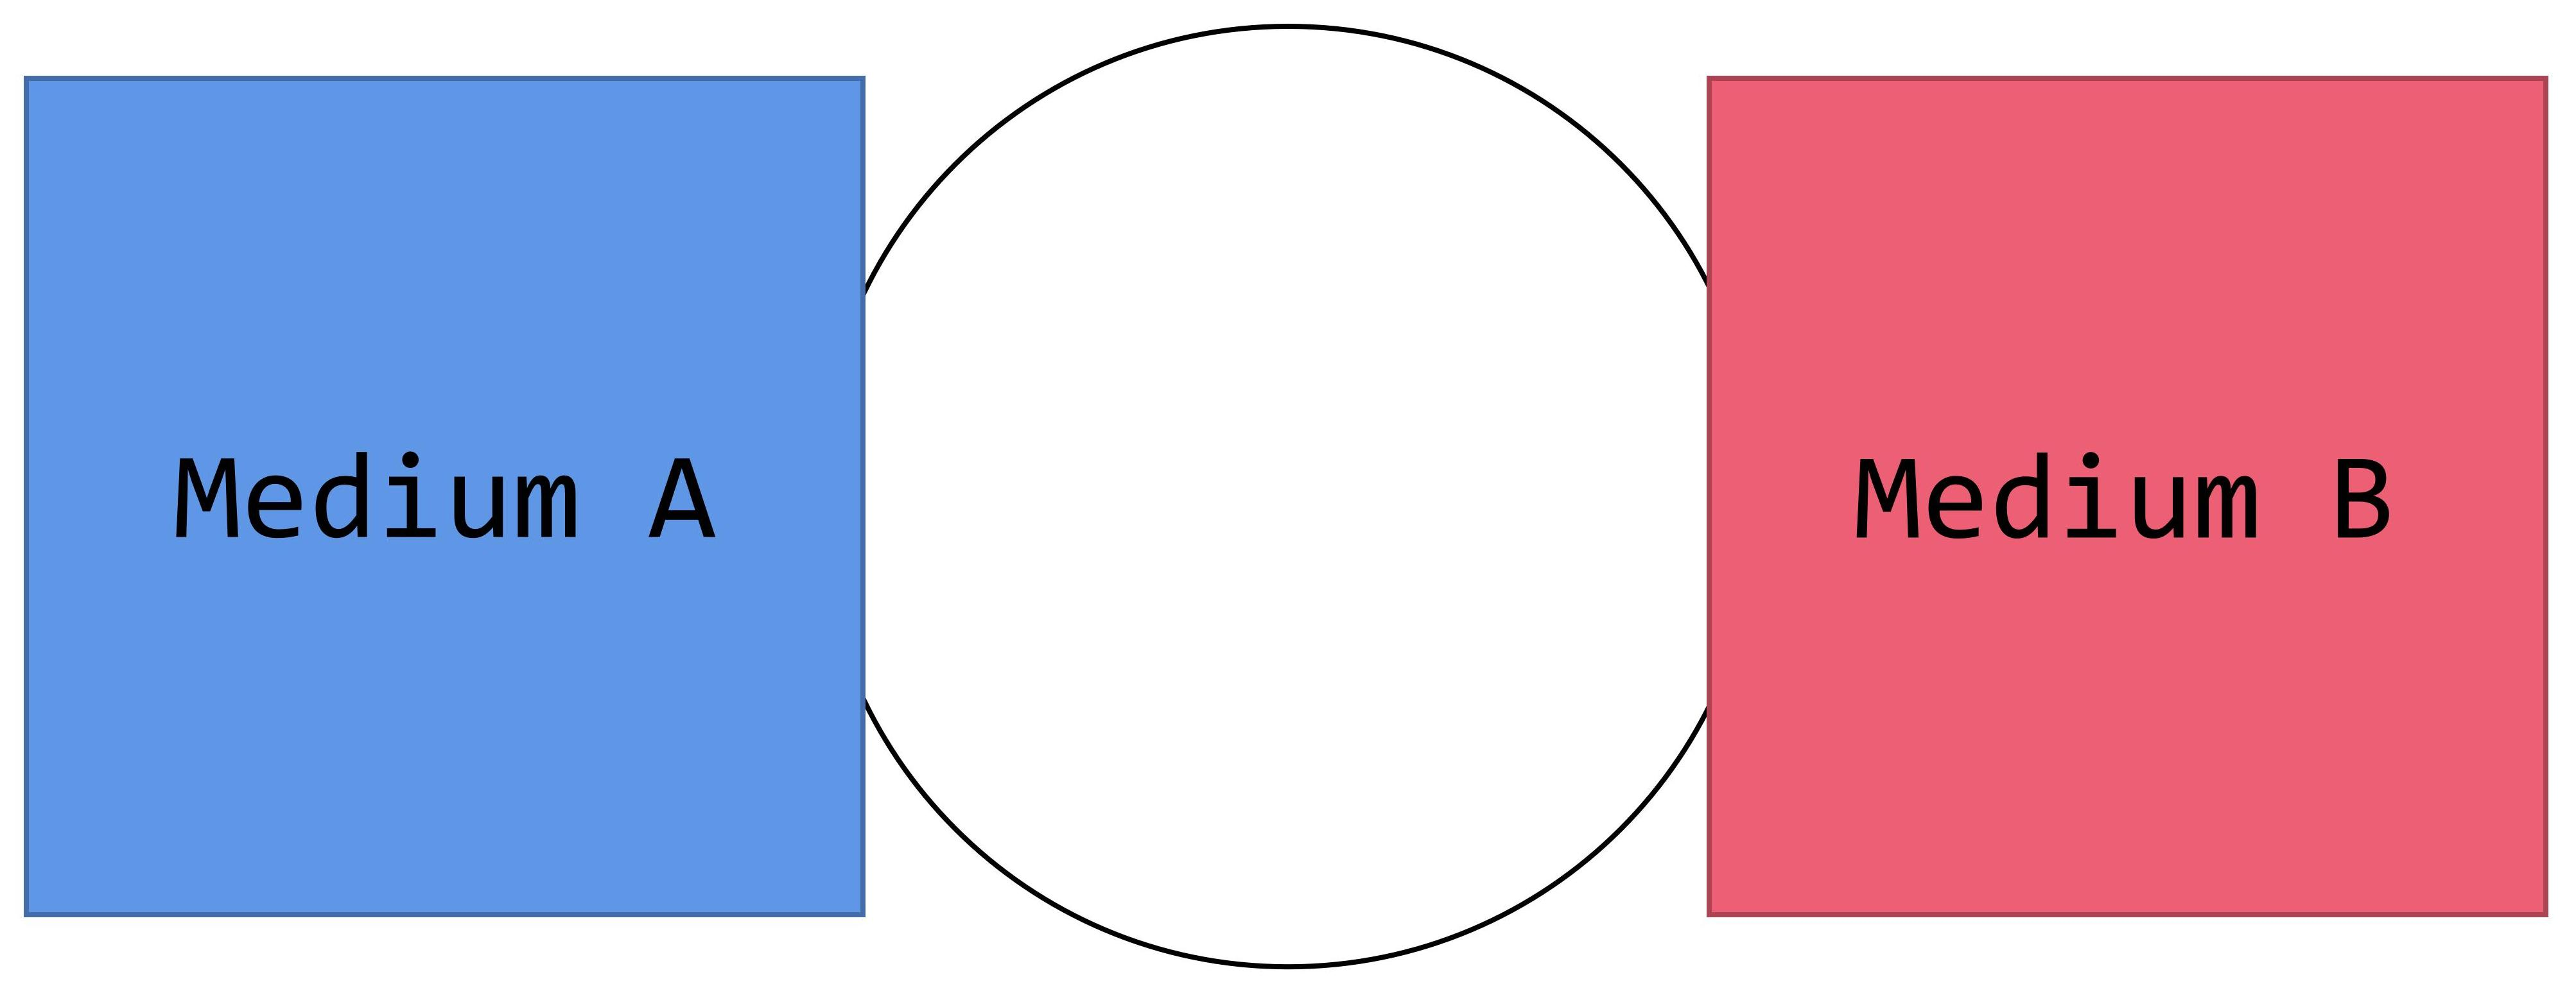
\includegraphics[scale=0.04]{pictures/surface weakness.png}
    \centering
    \caption{Weakness of the surface interface.}
\end{figure}
        Since `class Surface' contains only one pointer for the internal and external medium, 
    it is impossible to handle this two-medium case.
    So the middle sphere has to be split into two hemispheres.
\begin{figure}[H]
    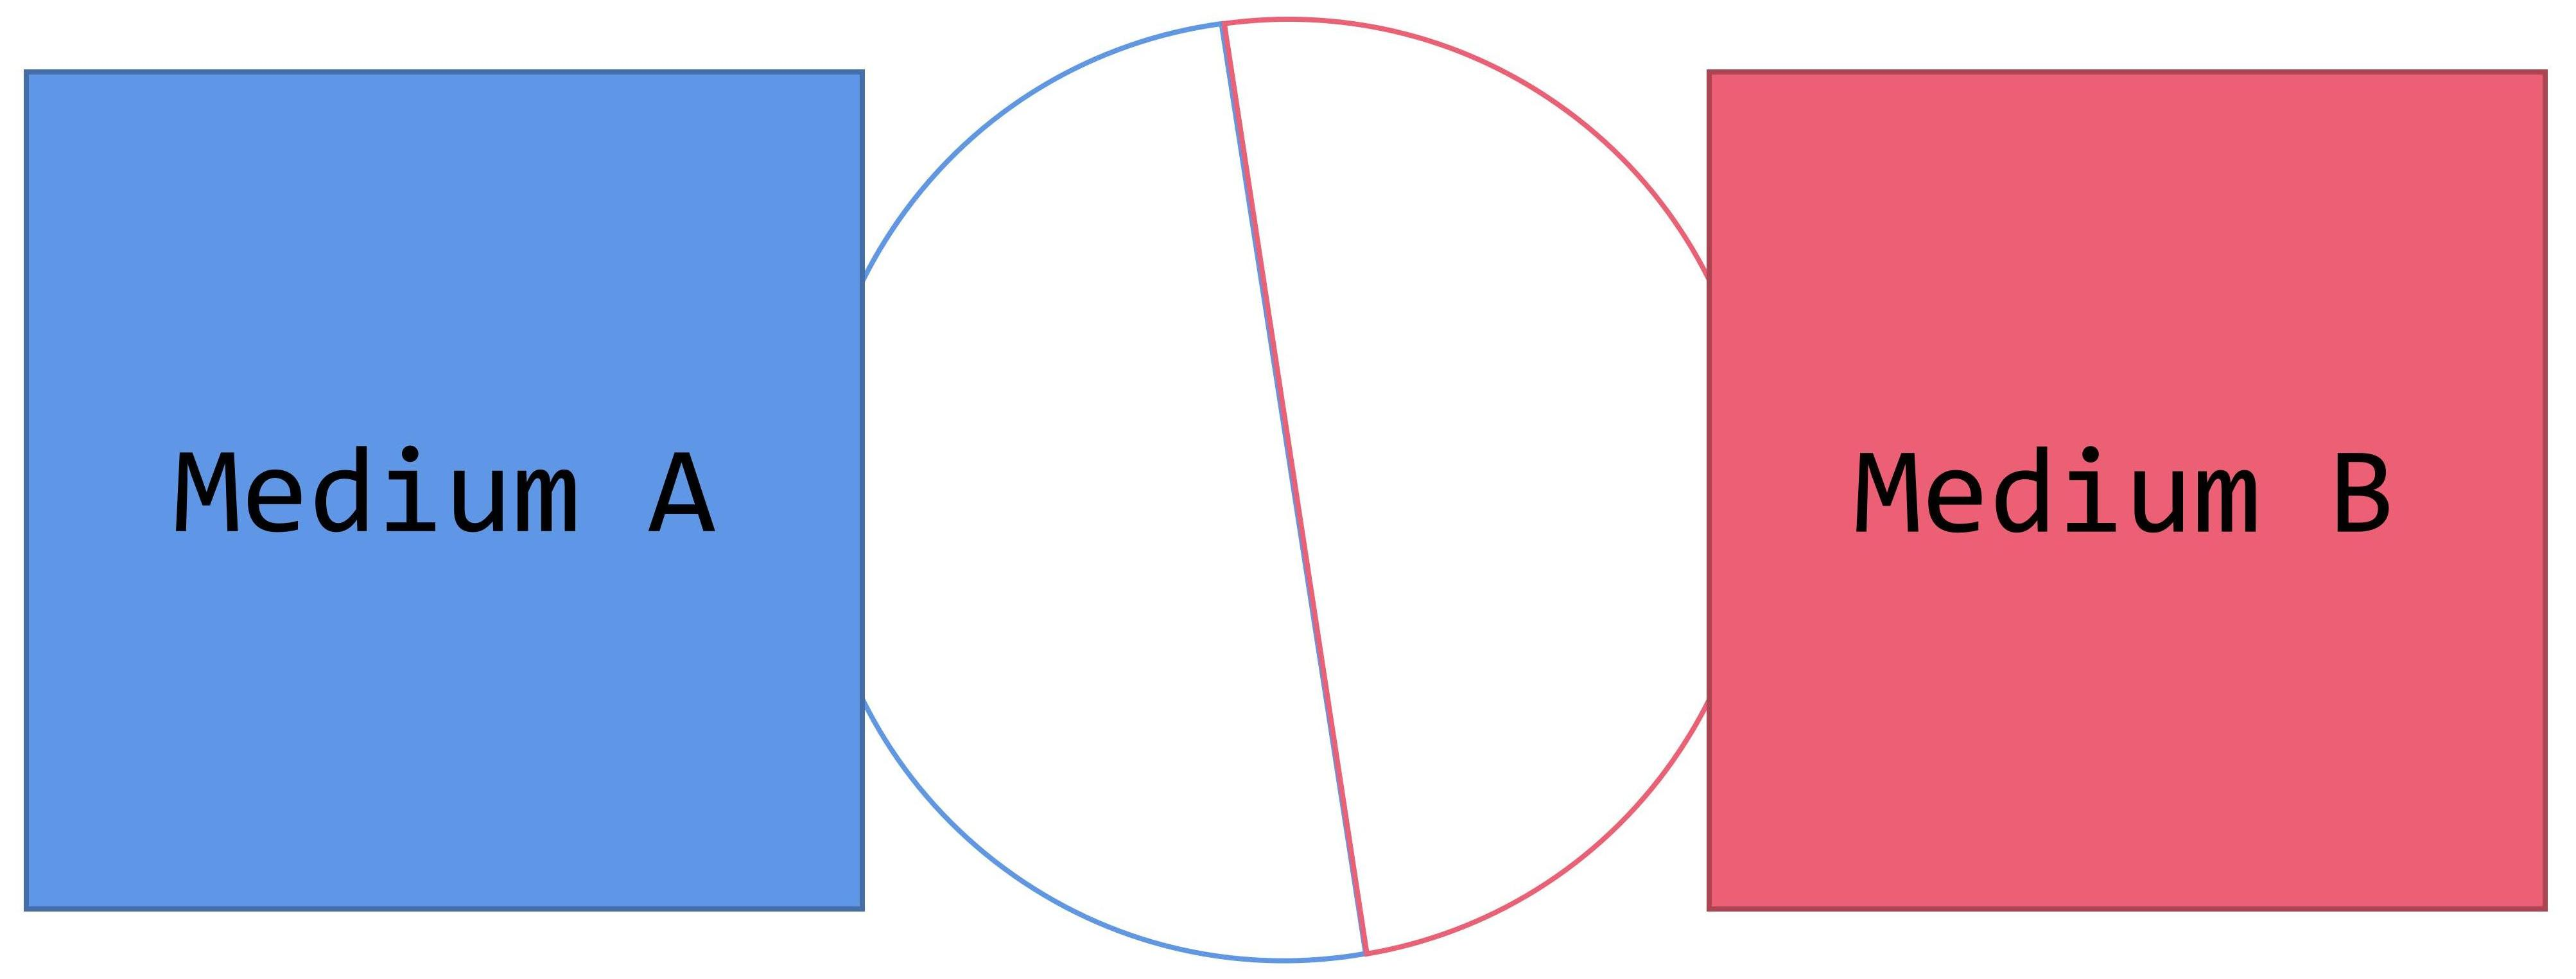
\includegraphics[scale=0.04]{pictures/surface weakness solution.png}
    \centering
    \caption{Solution to the weakness of the surface interface.}
\end{figure}
        Now that the data structures of the framework is clear, we will continue to the volume path tracing integrator.

\subsection{Integrator}
    See `volumePathSamplerIntegrator.h', `volumePathSamplerIntegrator.cpp' for more details.\par
        While `class SamplerIntegrator' implements `void Render()' to handle the rendering of an image, 
    every child classes derived form `class SamplerIntegrator' should implement `Spectrum Integrate()' to evaluate the radiance of a given ray casted to the scene.
    The method `Spectrum Integrate()' shares the similar meaning with `Spectrum Li()' in PBRT.\par
        To extend surface path tracing to volume path tracing, we first introduce the assumptions (restrictions) of our implementation.
    Then, we will mathematically prove the correctness of our integrator.
    Finally, we will explain the details of the implementation.
\subsubsection{Assumptions}
        It is difficult to implement emissive mediums because of the complicity to randomly sample a volume light.
    Even the mathematical proof will be much more complicated, 
    so we assume that all mediums are non-emissive.
\subsubsection{Mathematics}
        We start from volume rendering equation (VRE) with surface contributions.
\begin{equation} \label{eq1}
\begin{split}
    L(\x,\w) &= \int_0^z T(\x,\y)[\mu_a(\y)L_e(\y,\w)+\mu_s(\y)L_s(\y,\w)]dy\\
             &+T(\x,\z)L(\z,\w)
\end{split}
\end{equation}
    For non-emissive mediums, $L_e(\y,\w)=0$, so
\begin{equation} \label{eq2}
\begin{split}
    L(\x,\w) = \int_0^z T(\x,\y)\mu_s(\y)L_s(\y,\w)dy+T(\x,\z)L(\z,\w)
\end{split}
\end{equation}
    where
\begin{equation} \label{eq3}
\begin{split}
    L_s(\y,\w) = \int_{S^2}f_p(\w,\bar{\w})L(\y,\bar{\w})d\bar{\w}
\end{split}
\end{equation}
    Suppose camera is located at position $\p_0$, $\p_1$ is the first sampled position.
    Similarly define $\p_2, \p_3, \cdots$.
\begin{figure}[H]
    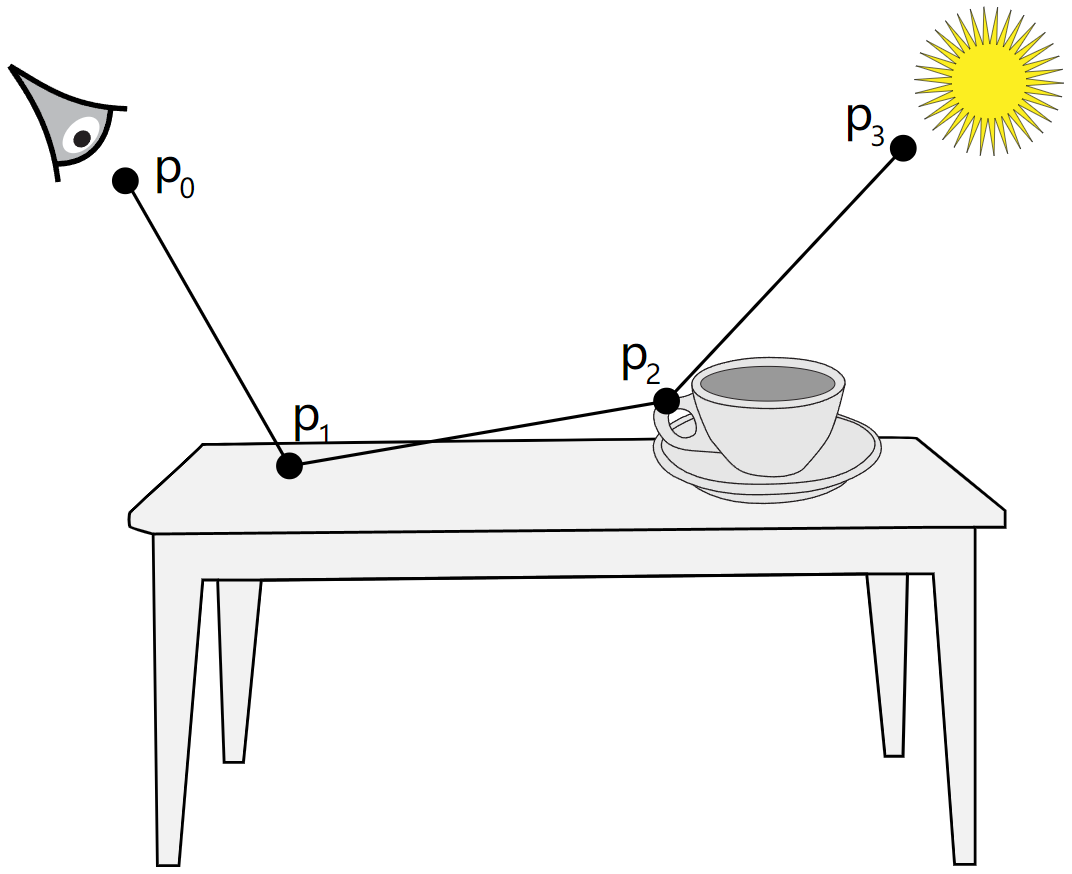
\includegraphics[scale=0.1]{pictures/path tracing.png}
    \centering
    \caption{Path tracing.}
\end{figure}
    For path tracing, we firstly consider only the two simplest cases: 
    both $\p_i,\p_{i+1}$ are in the air (no medium) and both $\p_i,\p_{i+1}$ are in some medium.
    Similar to the proof of surface path tracking in PBRT, we will derive the iteration of $\beta$ and `UniformSampleOneLight()' of these two cases.
    These two situations will be extended to more complicated cases later.\par
        For the first case where both $\p_i,\p_{i+1}$ are in the air, taking $\p_0,\p_1$ as an example.
\begin{equation} \label{eq4}
\begin{split}
    L(\pp{1}{0}) &= L_e(\pp{1}{0}) + L_r(\pp{1}{0})\\
                 &= L_e(\pp{1}{0})\\
                 &+ \int_{H^2(n)}L(\bar{\p}\rightarrow\p_1)f_r(\bar{\p}\rightarrow\p_1\rightarrow\p_0)|\mathrm{cos}\bar{\theta}|d\bar{\w}
\end{split}
\end{equation}
    where $L_e$ is the direct illumination from position $\p_1$ to position $\p_0$, 
    $L_r$ is the indirect illumination from position $\p_1$ to position $\p_0$.
    It should be noticed that $\bar{\p}$ is not ensured to be in air or in some medium so that 
    domain of $\bar{\p}$ should be split to those in air (on another surface), donated as $\bar{\p}^s$ and those in some medium, donated as $\bar{\p}^m$.
\begin{equation} \label{eq5}
\begin{split}
    L(\pp{1}{0}) &= L_e(\pp{1}{0})\\
                 &+ \int_{H^2(n)}L(\bar{\p}^s\rightarrow\p_1)f_r(\bar{\p}^s\rightarrow\p_1\rightarrow\p_0)|\mathrm{cos}\bar{\theta}|d\bar{\w}\\
                 &+ \int_{H^2(n)}L(\bar{\p}^m\rightarrow\p_1)f_r(\bar{\p}^m\rightarrow\p_1\rightarrow\p_0)|\mathrm{cos}\bar{\theta}|d\bar{\w}
\end{split}
\end{equation}
    where $L(\bar{\p}^s\rightarrow\p_1)$ can be evaluated using the surface contribution part of VRE and 
    $L(\bar{\p}^m\rightarrow\p_1)$ can be evaluated using the volume contribution part of VRE.
\begin{equation} \label{eq6}
\begin{split}
    L(\bar{\p}^s\rightarrow\p_1) &= T(\bar{\p}^s,\p_1)L_e(\bar{\p}^s\rightarrow\p_1)+T(\bar{\p}^s,\p_1)L_r(\bar{\p}^s\rightarrow\p_1)\\
    L(\bar{\p}^m\rightarrow\p_1) &= \int_{\p_1}^{\bar{\p}^m}T(\p_1,\p)\mu_s(\p)L_s(\p,\w_{\bar{\p}^m\rightarrow\p_1})ds
\end{split}
\end{equation}
    Substitute $L(\bar{\p}^s\rightarrow\p_1)$ into the path tracing equation.
\begin{equation} \label{eq7}
\begin{split}
    &\quad L(\pp{1}{0})\\
    &= L_e(\pp{1}{0})\\
    &+ \int_{H^2(n)} T(\bar{\p}^s,\p_1)L_e(\bar{\p}^s\rightarrow\p_1) f_r(\bar{\p}^s\rightarrow\p_1\rightarrow\p_0)|\mathrm{cos}\bar{\theta}|d\bar{\w}\\
    &+ \int_{H^2(n)} T(\bar{\p}^s,\p_1)L_r(\bar{\p}^s\rightarrow\p_1) f_r(\bar{\p}^s\rightarrow\p_1\rightarrow\p_0)|\mathrm{cos}\bar{\theta}|d\bar{\w}\\
    &+ \int_{H^2(n)} L(\bar{\p}^m\rightarrow\p_1) f_r(\bar{\p}^m\rightarrow\p_1\rightarrow\p_0)|\mathrm{cos}\bar{\theta}|d\bar{\w}
\end{split}
\end{equation}
    Apply Monte Carlo to the above equation.
\begin{equation} \label{eq8}
\begin{split}
    &\quad L(\pp{1}{0})\\
    &= L_e(\pp{1}{0})\\
    &+ \frac{T(\bar{\p}^s_{light},\p_1)L_e(\bar{\p}^s_{light}\rightarrow\p_1) f_r(\bar{\p}^s_{light}\rightarrow\p_1\rightarrow\p_0)|\mathrm{cos}\bar{\theta}|}{p(\w_{light})}\\
    &+
    \left\{\begin{aligned}
        \frac{L_r(\bar{\p}^s_{bsdf}\rightarrow\p_1)f_r(\bar{\p}^s_{bsdf}\rightarrow\p_1\rightarrow\p_0)|\mathrm{cos}\bar{\theta}|}{p(\w_{bsdf})}\\
            \mathrm{sample\ in\ air}\\
        \frac{L(\bar{\p}^m_{bsdf}\rightarrow\p_1) f_r(\bar{\p}^m_{bsdf}\rightarrow\p_1\rightarrow\p_0)|\mathrm{cos}\bar{\theta}|}{p(\w_{bsdf})}\ \ \\
            \mathrm{sample\ in\ some\ medium}\\
    \end{aligned}\right.
\end{split}
\end{equation}
    Define function
\begin{equation} \label{eq9}
\begin{split}
    &\ \mathrm{UniformSampleOneLight}(\pp{1}{0})\\
    &= \frac{T(\bar{\p}^s_{light},\p_1)L_e(\bar{\p}^s_{light}\rightarrow\p_1) f_r(\bar{\p}^s_{light}\rightarrow\p_1\rightarrow\p_0)|\mathrm{cos}\bar{\theta}|}{p(\w_{light})}
\end{split}
\end{equation}
    There is still a problem that it is difficult to evaluate $L(\bar{\p}^m_{bsdf}\rightarrow\p_1)$ because 
    $\p_1$ is in the air while $\bar{\p}^m_{bsdf}$ is in the medium.
    This problem can be solved by applying energy conservation while radiance is travelling in the air.\par
        Since $\bar{\p}^m_{bsdf}$ is in the medium and $\p_1$ is in the air, 
    there exists a position where radiance travels exactly from medium to the air.
    Take this picture as an example.
\begin{figure}[H]
    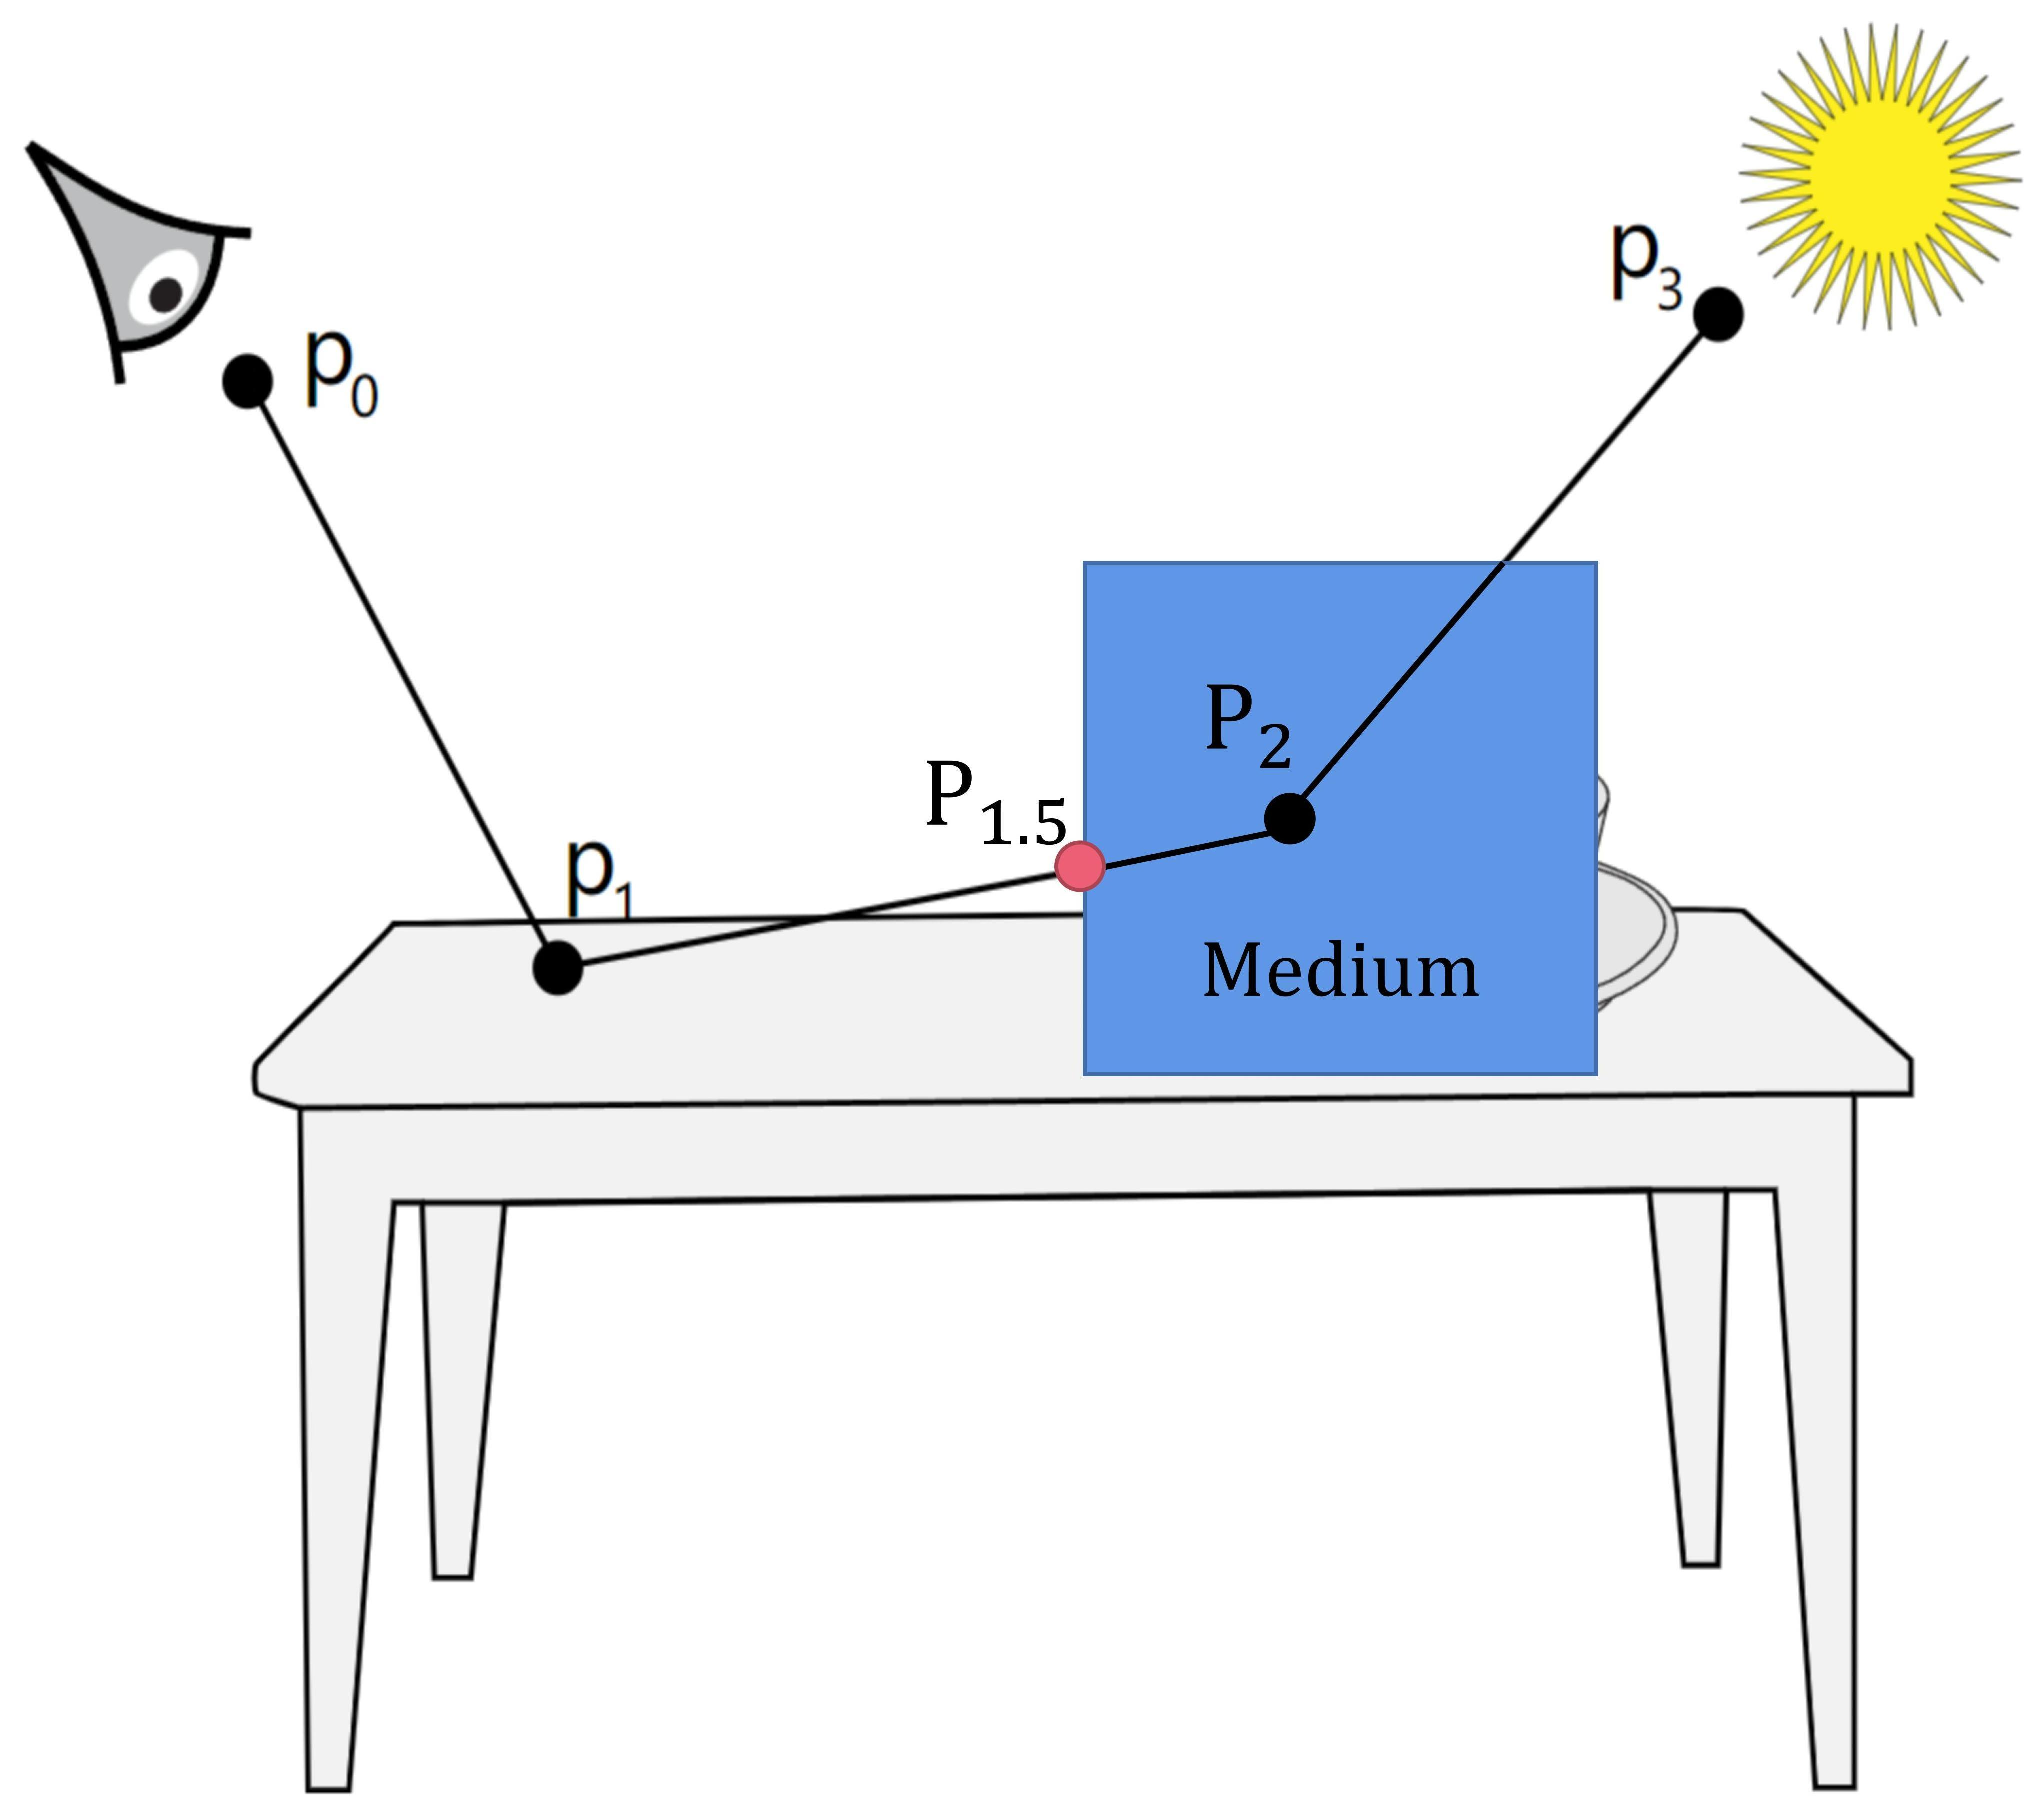
\includegraphics[scale=0.045]{pictures/volume path tracing.jpg}
    \centering
    \caption{Path tracing.}
\end{figure}
    Let $\p_{1.5}$ be the boundary between volume and air, apply energy conservation.
\begin{equation} \label{eq10}
\begin{split}
    L(\bar{\p}^m_{bsdf}\rightarrow\p_1) = L(\pp{1.5}{1})
\end{split}
\end{equation}
    Then the problem is converted from evaluating radiance from medium to air, to evaluating radiance from medium to medium
    because the boundary can be both considered as an in-air position and an in-medium position.\par
        The mathematics about evaluating radiance from medium to medium will be discussed then, 
    which is exactly the second case discussed above where both $\p_i,\p_{i+1}$ are in the air.
    Again take $\p_0,\p_1$ as an example.
    For in-medium case, $\p_1$ is got by sampling distance, so we donate $\p=\p_1$ below.
\begin{equation} \label{eq11}
\begin{split}
    &\ L(\pp{}{0})\\
    &= \int_{\p_0}^{\p}T(\p_0,\p)\mu_s(\p)L_s(\pp{}{0})ds\\
    &= \int_{\p_0}^{\p}T(\p_0,\p)\mu_s(\p)\int_{S^2}f_p(\bar{\p}\rightarrow\p\rightarrow\p_0)L(\bar{\p}\rightarrow\p)d\bar{\w}ds
\end{split}
\end{equation}
    Similar to the in-air case, $\bar{\p}$ is not ensured to be in air or in some medium.
\begin{equation} \label{eq12}
\begin{split}
    &\ L(\pp{}{0})\\
    &= \int_{\p_0}^{\p}T(\p_0,\p)\mu_s(\p)\int_{S^2}f_p(\bar{\p}^s\rightarrow\p\rightarrow\p_0)L(\bar{\p}^s\rightarrow\p)d\bar{\w}ds\\
    &+ \int_{\p_0}^{\p}T(\p_0,\p)\mu_s(\p)\int_{S^2}f_p(\bar{\p}^m\rightarrow\p\rightarrow\p_0)L(\bar{\p}^m\rightarrow\p)d\bar{\w}ds\\
    &= \int_{\p_0}^{\p}T(\p_0,\p)\mu_s(\p)\int_{S^2}f_p(\bar{\p}^s\rightarrow\p\rightarrow\p_0)\\
    &\quad\quad\quad \left(T(\bar{\p}^s,\p)L_e(\bar{\p}^s\rightarrow\p)+T(\bar{\p}^s,\p)L_r(\bar{\p}^s\rightarrow\p)\right)d\bar{\w}ds\\
    &+ \int_{\p_0}^{\p}T(\p_0,\p)\mu_s(\p)\int_{S^2}f_p(\bar{\p}^m\rightarrow\p\rightarrow\p_0)L(\bar{\p}^m\rightarrow\p)d\bar{\w}ds
\end{split}
\end{equation}
    Apply Monte Carlo for sampling scattering distance.
\begin{equation} \label{eq13}
\begin{split}
    &\ L(\pp{}{0})\\
    &= \frac{T(\p_0,\p)\mu_s(\p)}{p({\p})}\int_{S^2}f_p(\bar{\p}^s\rightarrow\p\rightarrow\p_0)T(\bar{\p}^s,\p)L_e(\bar{\p}^s\rightarrow\p)d\bar{\w}\\
    &+ \left\{\begin{aligned}
            \frac{T(\p_0,\p)\mu_s(\p)}{p({\p})}\int_{S^2}f_p(\bar{\p}^s\rightarrow\p\rightarrow\p_0)T(\bar{\p}^s,\p)L_r(\bar{\p}^s\rightarrow\p)d\bar{\w}\\
            \mathrm{sample\ in\ air}\\
            \frac{T(\p_0,\p)\mu_s(\p)}{p({\p})}\int_{S^2}f_p(\bar{\p}^m\rightarrow\p\rightarrow\p_0)L(\bar{\p}^m\rightarrow\p)d\bar{\w}\quad\quad\quad \\
            \mathrm{sample\ in\ some\ medium}\\
        \end{aligned}\right.
\end{split}
\end{equation}
    It should be noticed that for those tracking methods derived from delta tracking, $p({\p})=T(\p_0,\p)\mu_t(\p)$. Then
\begin{equation} \label{eq14}
\begin{split}
    \frac{T(\p_0,\p)\mu_s(\p)}{p({\p})} = \frac{\mu_s(\p)}{\mu_t(\p)}.
\end{split}
\end{equation}
    Apply Monte Carlo for sampling scattering direction.
\begin{equation} \label{eq15}
\begin{split}
    &\ L(\pp{}{0})\\
    &= \frac{T(\p_0,\p)\mu_s(\p)}{p({\p})} \frac{f_p(\bar{\p}^s_{light}\rightarrow\p\rightarrow\p_0)T(\bar{\p}^s_{light},\p)L_e(\bar{\p}^s_{light}\rightarrow\p)}{p(\w_{light})}\\
    &+ \left\{\begin{aligned}
            \frac{T(\p_0,\p)\mu_s(\p)}{p({\p})} \frac{f_p(\bar{\p}^s_{phase}\rightarrow\p\rightarrow\p_0)T(\bar{\p}^s_{phase},\p)L_r(\bar{\p}^s_{phase}\rightarrow\p)}{p(\w_{phase})}\\
            \mathrm{sample\ in\ air}\\
            \frac{T(\p_0,\p)\mu_s(\p)}{p({\p})} \frac{f_p(\bar{\p}^m_{phase}\rightarrow\p\rightarrow\p_0)L(\bar{\p}^m_{phase}\rightarrow\p)}{p(\w_{phase})}\quad\quad\quad\quad\quad\ \ \\
            \mathrm{sample\ in\ some\ medium}\\
        \end{aligned}\right.\\
    &= \frac{T(\p_0,\p)\mu_s(\p)}{p({\p})} \frac{f_p(\bar{\p}^s_{light}\rightarrow\p\rightarrow\p_0)T(\bar{\p}^s_{light},\p)L_e(\bar{\p}^s_{light}\rightarrow\p)}{p(\w_{light})}\\
    &+ \left\{\begin{aligned}
            \frac{T(\p_0,\p)\mu_s(\p)}{p({\p})} T(\bar{\p}^s_{phase},\p)L_r(\bar{\p}^s_{phase}\rightarrow\p)\\
            \mathrm{sample\ in\ air}\\
            \frac{T(\p_0,\p)\mu_s(\p)}{p({\p})} L(\bar{\p}^m_{phase}\rightarrow\p)\quad\quad\quad\quad\quad\ \ \\
            \mathrm{sample\ in\ some\ medium}\\
        \end{aligned}\right.
\end{split}
\end{equation}
    Define function
\begin{equation} \label{eq16}
\begin{split}
    &\ \mathrm{UniformSampleOneLight}(\pp{}{0})\\
    &= \frac{T(\p_0,\p)\mu_s(\p)}{p({\p})} \frac{f_p(\bar{\p}^s_{light}\rightarrow\p\rightarrow\p_0)T(\bar{\p}^s_{light},\p)L_e(\bar{\p}^s_{light}\rightarrow\p)}{p(\w_{light})}
\end{split}
\end{equation}
    There is also a similar problem that it is difficult to evaluate $L_r(\bar{\p}^s_{phase}\rightarrow\p)$ because $\p$ is in some medium while $\bar{\p}^s_{phase}$ is in the air.
    This problem can also be solved similarly by energy conservation.\par
        For now, the two simplest cases (both $\p_i,\p_{i+1}$ are in the air or in some medium) has been solved.
    Readers may have noticed that it is quite easy to derive them into more complicated cases by using an empty BSDF for the wrapping surface of the medium.
    That is, ray simply travels through the wrapping surface without scattering.
    The following picture shows the idea.
\begin{figure}[H]
    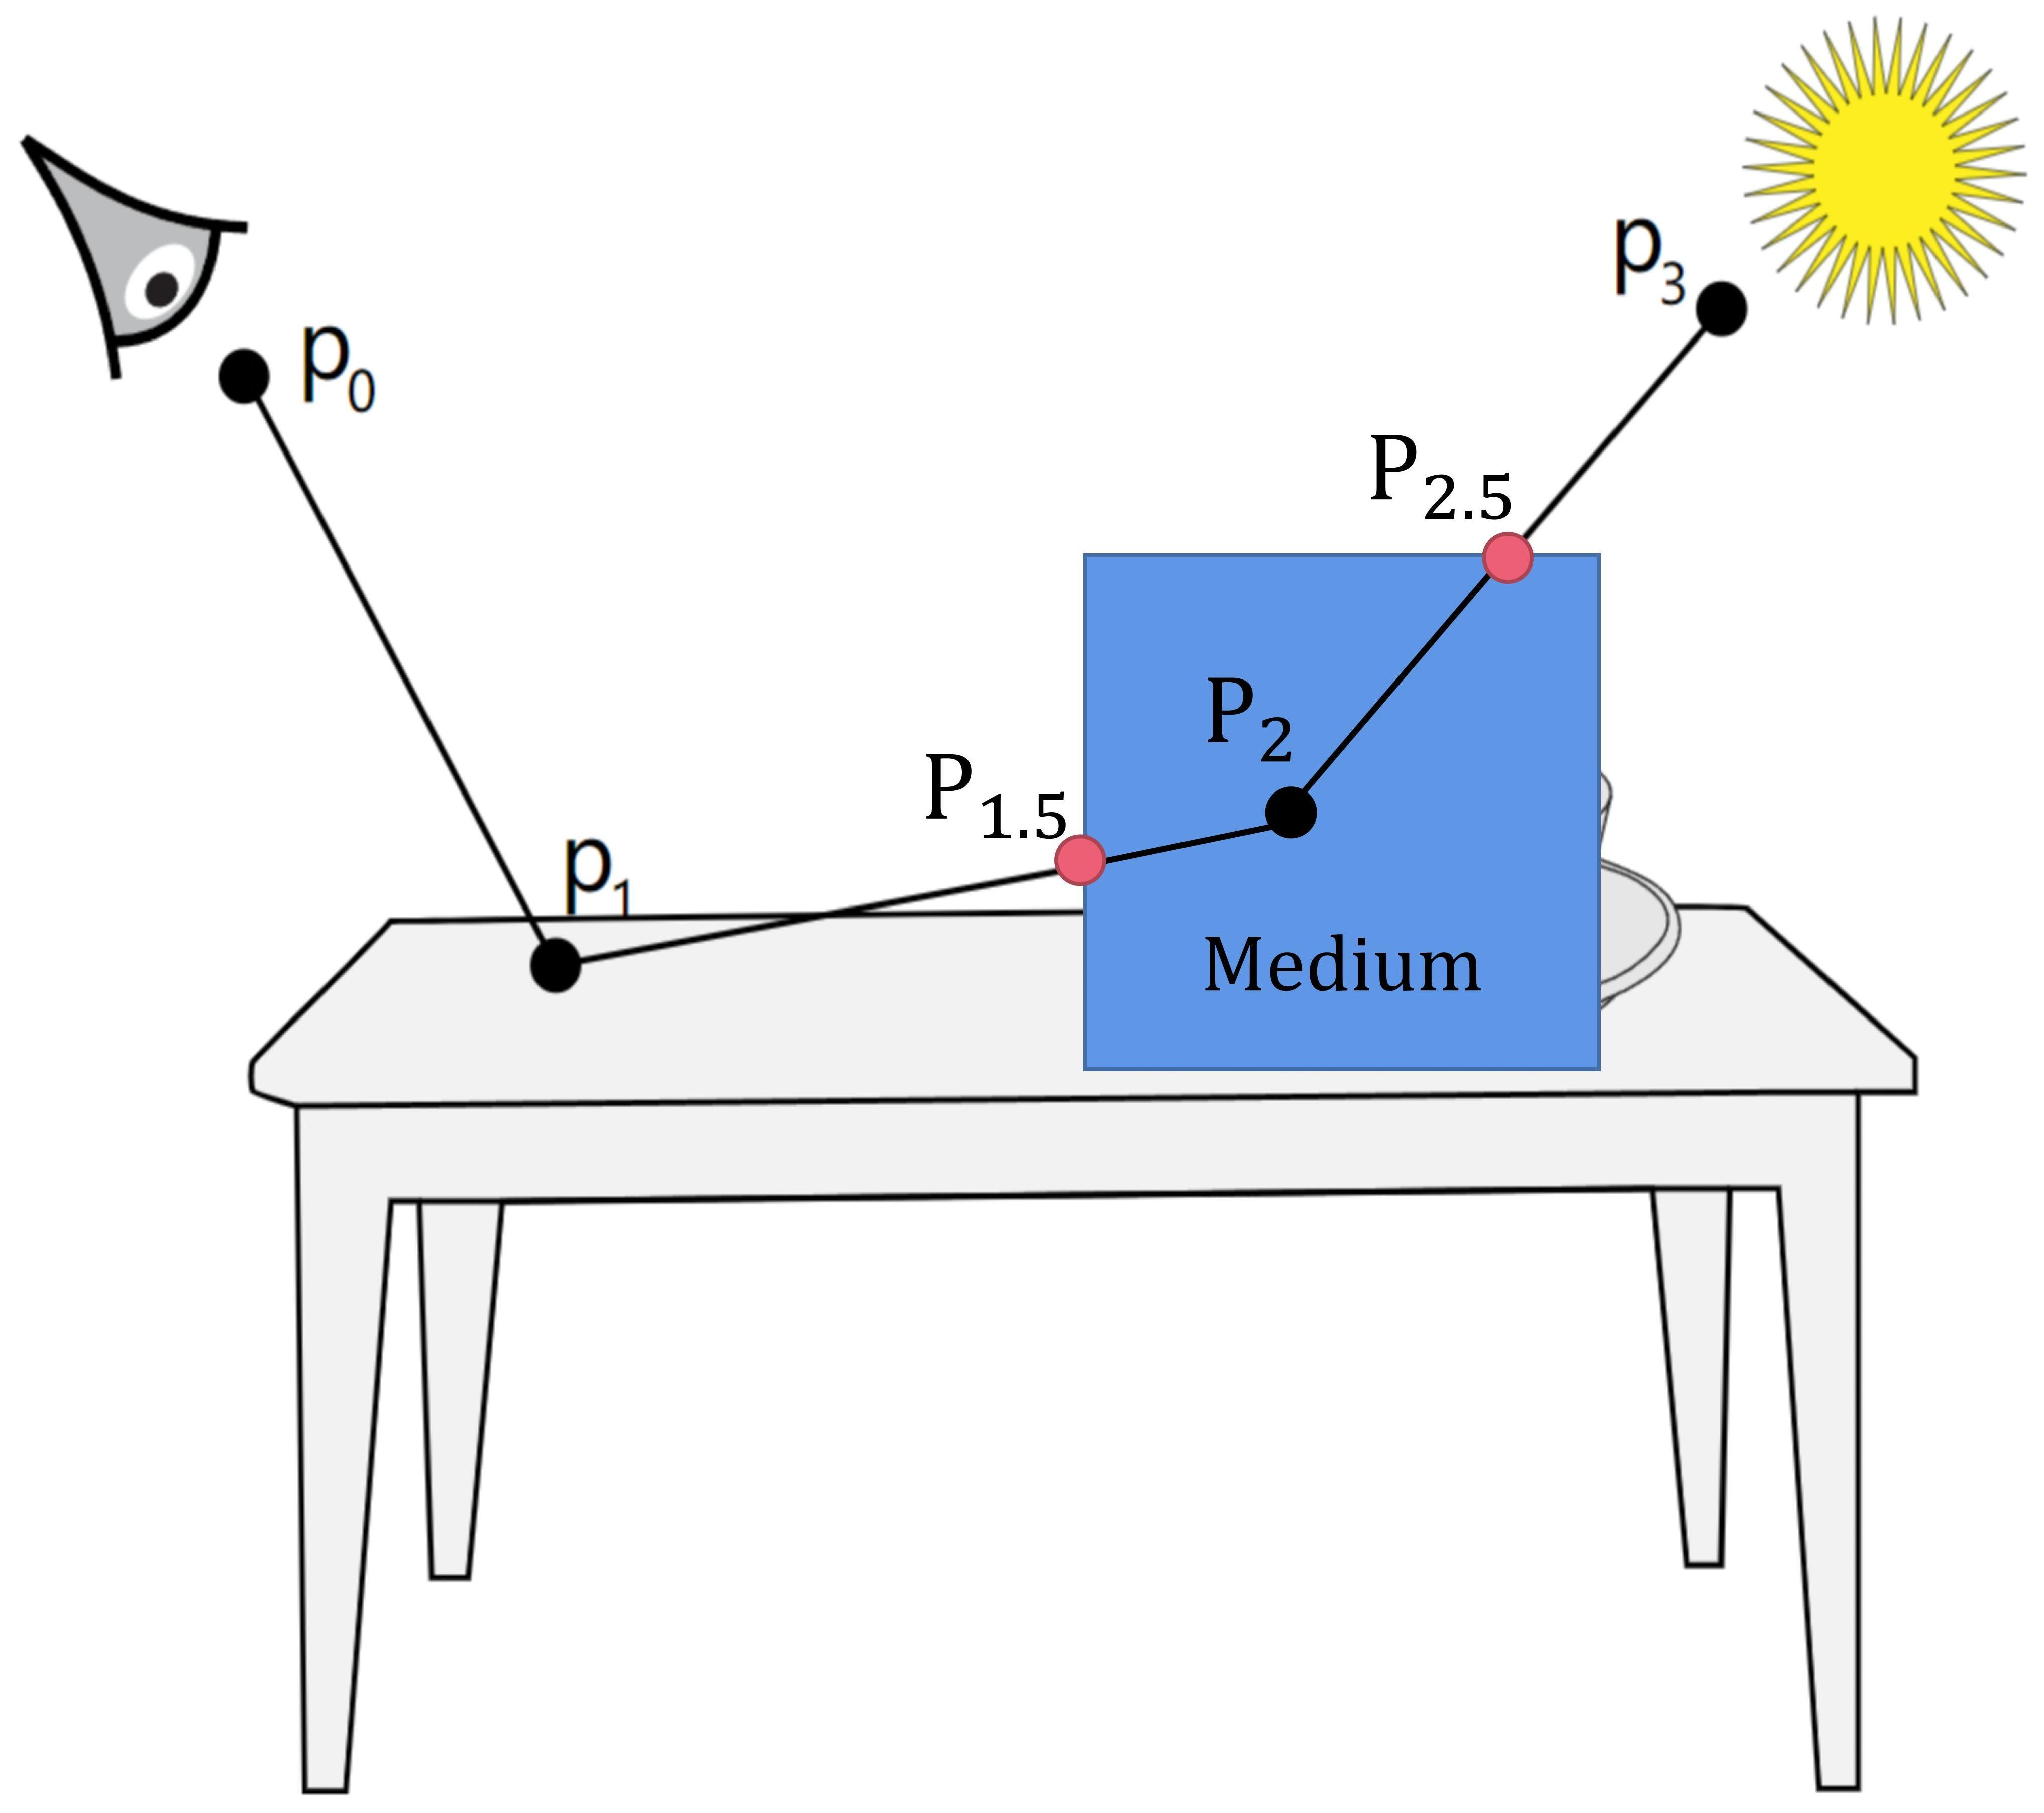
\includegraphics[scale=0.045]{pictures/volume path tracing ultimate.jpg}
    \centering
    \caption{Ultimate volume path tracing.}
\end{figure}
    Path $\p_3\rightarrow\p_2\rightarrow\p_1\rightarrow\p_0$ is extended to $\p_3\rightarrow\p_{2.5}\rightarrow\p_2\rightarrow\p_{1.5}\rightarrow\p_1\rightarrow\p_0$, 
    then nodes of each single path are located both in the air or in some medium.
    It is valid to combine them together, which derives our integrator for volume rendering.\par
        Now we will derive the iteration of $\beta$ and `UniformSampleOneLight()', which is clearly proved above.
\begin{equation} \label{eq17}
\begin{split}
    \beta(i) = \prod_{j=1}^{i}
        \left\{\begin{aligned}
            \frac{f_r(\p_{j+1}\rightarrow\p_{j}\rightarrow\p_{j-1})|\mathrm{cos}\theta_j|}{p_\w(\p_{j+1}\rightarrow\p_j)}\quad\ \ \mathrm{sample\ in\ air}\\
            \frac{T(\p_j,\p_{j+1})\mu_s(\p_{j+1})}{p({\p_{j+1}})}\quad \mathrm{sample\ in\ some\ medium}\\
        \end{aligned}\right.\\
\end{split}
\end{equation}
\begin{equation} \label{eq18}
\begin{split}
    &\ \mathrm{UniformSampleOneLight}(\pp{j}{j-1})\\
    &=  \left\{\begin{aligned}
            \frac{T(\bar{\p}^s_{light},\p_j)L_e(\bar{\p}^s_{light}\rightarrow\p_j) f_r(\bar{\p}^s_{light}\rightarrow\p_j\rightarrow\p_{j-1})|\mathrm{cos}\bar{\theta}|}{p(\w_{light})}\\
            \mathrm{sample\ in\ air}\\
            \frac{T(\p_{j-1},\p_j)\mu_s(\p_j)}{p({\p_j})}\cdot\quad\quad\quad\quad\quad\quad\quad\quad\quad\quad\quad\quad\quad\quad\quad\quad\ \\
            \frac{f_p(\bar{\p}^s_{light}\rightarrow\p_j\rightarrow\p_{j-1})T(\bar{\p}^s_{light},\p_j)L_e(\bar{\p}^s_{light}\rightarrow\p_j)}{p(\w_{light})}\quad\quad\ \\
            \mathrm{sample\ in\ some\ medium}\\
        \end{aligned}\right.\\
\end{split}
\end{equation}
    Then the radiance of a pixel can be determined.
    For surface path tracing, the radiance of a pixel can be rewritten to the following iterative equation.
\begin{equation} \label{eq19}
\begin{split}
    \mathrm{radiance} &= L_e(\pp{1}{0})\\
                      &+ \beta_0\mathrm{UniformSampleOneLight(\pp{1}{0})}\\
                      &+ \beta_1\mathrm{UniformSampleOneLight(\pp{2}{1})}\\
                      &+ \cdots
\end{split}
\end{equation}
    For volume path tracing, the iterative equation is too complicated to be described by mathematics so it will not be shown here.

\subsubsection{Implementation}
    The implementation simply translate the above mathematics into code.
    Readers may find that our implementation is quite similar to PBRT.
    That is right because we accidentally chose the similar implementation approach with PBRT (but PBRT does not prove the correctness of their implementation).
    We will further discuss the restriction of PBRT and show the better implementation in the next section 
    while introducing spectral weighed delta tracking and spectral weighed decomposition tracking.\par
        Here is the pseudo code written with PBRT literate programming.
\lstset{basicstyle=\tiny\ttfamily}
\begin{lstlisting}
Spectrum
VolumePathSamplerIntegrator::Integrate(const Ray& r, const Scene& scene) const:
  Spectrum radiance(Float(0));
  Ray ray(r);
  bool specularBounce = false;
  Spectrum beta(Float(1));
  Spectrum mediumScatteringWeigh(Float(1));
  const Medium* medium = camera->medium;
  for (int bounces = 0; ; ++bounces):
    <<Intersect ray with scene and store intersection in si>>
    <<Sample the participating medium and store intersection in mi, if present>>
    // Handle an interaction with a medium or a surface
    if (mi.IsValid()):
      // Handle scattering at point in medium for volumetric path tracer
      radiance += beta * UniformSampleOneLight(...);
      <<Spawn ray from mi>>
    else:
      // Handle scattering at point on surface for volumetric path tracer
      <<Possibly add emitted light at intersection>>
      <<Terminate path if ray escaped or max depth was reached>>
      // Compute scattering functions and skip over medium boundaries>>
      si.ComputeScatteringFunctions(ray);
      if (!si.bsdf):
        <<Spawn ray from si>>
        --bounces;
        continue;
      // Sample illumination from lights to find attenuated path contribution
      radiance += beta * UniformSampleOneLight(...);
      <<Sample BSDF to get new path direction>>
    <<Possibly terminate the path with Russian roulette>>
  return radiance;
\end{lstlisting}
\lstset{basicstyle=\small\ttfamily}
    For the integrator to run successfully, child classes of `class Medium' should be implemented then, 
    which will be introduced in the next section.

\subsection{Density Medium}
    See `densityMedium.h', `densityMedium.cpp' for more details.\par
        Information of volumes can be described by a floating point grid called density, 
    accompanied by some mega information to translate density into $\mu_a, \mu_s, \mu_t$.\par
        It should be noticed that even density at a given position is simply a floating point, 
    $\mu_a, \mu_s, \mu_t$ are spectrums.
    That is, they are wavelength-interdependent.
    So that spectral tracking (weighed delta tracking and weighed decomposition tracking) should be used.
    Readers familiar with PBRT may be confused since PBRT implements non-weighed delta tracking.
    That is because PBRT does not support wavelength-interdependent $\mu_t$.
    See the source code of PBRT for more details.\par
        In this section, we are proud to extend PBRT by implementing wavelength-interdependent mediums.
    We will first introduce the fields of the classes.
    We will then explain how to sample scattering distance and evaluate transmittance for mediums based on grid and KDTree.

\subsubsection{Fields of Classes}
    Density is interpreted as $\mu_t$ in our implementation so the first step is to transform density to $\mu_t$.
    This is done by providing a spectrum called `toMut', then $\mu_t=\mathrm{density\cdot toMut}$.
    $\mathrm{Albedo}=\frac{\mu_s}{\mu_t}$ should also be provided to compute $\mu_a$ and $\mu_s$ from $\mu_t$.
    Such an idea derives the interfaces of density mediums.
\begin{lstlisting}
class HeteroMedium : public Medium;
class DensityGridMedium : public HeteroMedium:
protected:
    const VolumeFloatGrid* density;
    const Spectrum toMut;
    const Spectrum albedo;
    const PhaseFunction* phase;
    const Transform worldToMedium;
class DensityKDTreeMedium : public HeteroMedium:
    ... // The same
\end{lstlisting}
    For delta tracking, $\bar{\mu}$ should be determined during the construction.
    Since density is given, we choose $\bar{\mu}=\mathrm{max}(\mathrm{density})$.
    $\frac{1}{\bar{\mu}}$ is also computed to make the sampling process faster.
\begin{lstlisting}
class DensityGridDeltaMedium : 
      public DensityGridMedium:
private:
    Float mubar;
    Float mubar_inv;
\end{lstlisting}
    For decomposition tracking, besides $\bar{\mu}$ and $\frac{1}{\bar{\mu}}$, 
    $\mu_a^c$, $\mu_s^c$, $\mu_t^c$, $P_a^c$, $P_s^c$, $P_{residual}$ should also be computed.
    Since it is not that easy to evaluate transmittance wavelength-interdependently by residual ratio tracking, 
    a homogeneous choice of $\mu_t^c$ should also be computed, as well as the corresponding $\frac{1}{\bar{\mu^r}}$.
\begin{lstlisting}
class DensityGridDecompositionMedium : 
      public DensityGridMedium:
private:
    Float mubar;
    Float mubar_inv;
    Spectrum muaC;
    Spectrum musC;
    Spectrum mutC;
    Float paC;
    Float psC;
    Float pResidual;
    Float mutC_homoC;
    Float mubarR_homoC_inv;
\end{lstlisting}

\subsubsection{Sampling Scattering Distance}
    As has mentioned above, we follow the similar interface for `Medium::Sample()'.
    That is, the return value is the updating multiplier for $\beta$, which is exactly $\frac{T(\p_{j-1},\p_j)\mu_s(\p_j)}{p({\p_j})}$.
    For tracking methods based on delta tracking including decomposition tracking, it can be simplified to $\frac{\mu_s(\p_j)}{\mu_t(\p_j)}$.
    Thus the return value is always the albedo.
    Our implementation assumes fixed albedo for a medium, different from PBRT.\par
        The code simply translates weighed delta tracking and weighed decomposition tracking of Disney pseudo code into C++, 
    except that `weigh' is a parameter.
    When a ray is scattering inside a medium weigh is updated during each scattering process, 
    until the ray finally travels out of the medium, then the weigh is reset to `Spectrum(Float(1))'.
    The weigh is kept in the integrator as a variable called `Spectrum mediumScatteringWeigh'.\par
        Problem occurs when there are solid shapes inside a medium.
    Delta tracking and transmittance evaluation should never overreach these shapes.
    So a ray casting always has to be performed before calls to functions `Sample()' and `Tr()' in order to record the maximum sampling distance inside `rayWorld.tMax'.
    `tMax' should also be recomputed when ray is transformed from world coordinate to grid coordinate, as readers will see in our source code.\par
        Pseudo code of weighed delta tracking for grid is shown here.
\lstset{basicstyle=\tiny\ttfamily}
\begin{lstlisting}
Spectrum
DensityGridDeltaMedium::Sample(
        const Ray& rayWorld, Sampler& sampler, 
        Spectrum* weigh, MediumInteraction* mi) const:
  <<Transform ray from world coordinate to grid coordinate>>
  <<Ray casting to the bounding box and compute tMin, tMin>>
  // Weighed delta tracking
  Float t = tMin;
  while (true):
    // Step forward
    t -= std::log(1 - sampler.Get1D()) * mubar_inv;
    if (t > tMax):
      break;
    <<Compute sampling variables such as Pa, Ps, Pn>>
    if (kexi < pa):
      <<Set mi->emission>>
      return Spectrum(Float(0)); // Terminate path
    else if (kexi < 1 - pn):
      <<Update weigh>>
      <<Set mi>>
      return albedo; // Return albedo to update beta
    else:
      <<Update weigh>>
  return Spectrum(Float(1)); // Sampling failed
\end{lstlisting}
\lstset{basicstyle=\small\ttfamily}
    Code of weighed decomposition tracking for grid is shown in `DensityGridDecompositionMedium::Sample()', 
    which is quite similar so it will be shown here.\par
        Tracking for KDTree is also straightforward.
    Readers can simply replace the intersection testing of traversal of PBRT KDTree with node-level delta tracking or decomposition tracking.
    But it should be noticed that if a real collision is sampled inside one node, other nodes should no longer be sampled, 
    which is different from a KDTree containing primitives because a primitive may be located inside many nodes but a medium-grid block is located inside exactly one node.\par
        The codes of `DensityKDTreeDeltaMedium::Sample()' and `DensityKDTreeDecompositionMedium::Sample()' is so simple that they will also not be included here.

\subsubsection{Evaluating transmittance}
    Since ratio tracking is related to weighed delta tracking and residual ratio tracking is related to weighed decomposition tracking.
    We use ratio tracking for "delta" medium and residual ratio tracking for "decomposition" medium.\par
        The following code shows the evaluation of transmittance by ratio tracking for grid.
\lstset{basicstyle=\tiny\ttfamily}
\begin{lstlisting}
Spectrum
DensityGridDeltaMedium::Tr(const Ray& rayWorld, Sampler& sampler) const:
  <<Transform ray from world coordinate to grid coordinate>>
  <<Ray casting to the bounding box and compute tMin, tMin>>
  // Ratio tracking
  while (true):
    // Step forward
    t -= std::log(1 - sampler.Get1D()) * mubar_inv;
    if (t >= tMax):
      break;
    Float dense = density->Sample(rayMedium(t));
    tr *= Spectrum(Float(1)) 
        - Spectrum::Max(Spectrum(), dense * mubar_inv * toMut);
  return tr;
\end{lstlisting}
\lstset{basicstyle=\small\ttfamily}
    However, for decomposition tracking, $\mu^c$ which is independent among wavelengths have to be used
    because those with interdependence is not supported by residual ratio tracking.\par
        The code for the other three cases are not shown since they share too much similarities.\par
        There is still one interface to implement for the integrator to comfortably evaluate transmittance.
    A ray may travel through many mediums before hitting a solid surface.
    For these cases, the accumulated transmittance should be evaluated.
    This is done by evaluating and multiplying the transmittance of all the mediums along the ray.
    So `IntersectTr()' is used instead of `Intersect()' in volume path tracing, 
    which evaluates the transmittance along the ray and returns whether the ray hits a solid surface.
    See `scene/scene.h', `scene/scene.cpp' for the details of the interface.
\begin{lstlisting}
Scene:IntersectTr(
    const Ray& ray,         // World-coord ray
    Sampler& sampler,       // Random generator
    const Medium* medium,   // Medium with ray.o
    Float* tHit,            // Hit time
    SurfaceInteraction* si, // Interaction info
    Spectrum* tr            // Transmittance
);
\end{lstlisting}
    Now we are done.

\subsection{Aggregate}
    See `embreeAccel.h', `embreeAccel.cpp' for more details.\par
    Since volume global illumination is quite slow, we provide an accelerator based on Intel Embree.
    The scenes are rendered with `embreeAccel' in default for performance, 
    but we also provide interfaces for our self-written accelerators including KDTree and BVH.
\begin{lstlisting}
#ifdef INTEL
shared_ptr<EmbreeAccel> aggregate = 
    make_shared<EmbreeAccel>(primitives);
#else
shared_ptr<BVH> aggregate = 
    make_shared<BVH>(primitives);
#endif
\end{lstlisting}
    Readers can enable or disable Embree by setting `INTEL' in cmake.
\begin{lstlisting}
set(INTEL true)
\end{lstlisting}

\section{TODO}
    We failed to implement everything because time is limited.
    Features not yet implemented are introduced in this section.
\subsection{Emissive Medium}
    Has been proved above, our integrator does not support emissive medium.
    A better integrator should be mathematically proved.
\subsection{Faster IntersectTr()}
    The function `IntersectTr()' is quite slow because it may calls `Intersect()' multiple times when there are multiple mediums in the scene.
    This can be solved by using Embree interfaces about masking.
\subsection{MIS}
    We haven't updated the MIS for surface rendering to volume rendering because
    some interfaces of the framework have been updated to support volume rendering, 
    so that MIS has to be written.
\subsection{Better Interface for Surface}
    Has also been mentioned above, it is difficult for our interface to handle overlaps of solid shapes and mediums.
    A special pointer texture may be a solution, but storing and looking up such a texture may be expensive.
\subsection{Packet Tracking}
    Since our implementation is originally not based on Embree, it does not support packet tracking very well.
    To implementation this feature, the whole framework should be rewritten.
\subsection{Handling Floating Point Errors}
    PBRT restrictedly handle floating point errors especially nans.
    It is extremely important when rays are frequently bounced from surfaces
    because infinite loops will occur if rays are not correctly bounced.

\section{Results}

\end{document}
